\section{Graphische Benutzungsoberflächen - Kontrollfragen}
\subsection{Begriffe und Geschichte}
\begin{enumerate}
	\item Erläutern Sie die Begriffe Dialogsystem, UI und Usability!
	\begin{itemize}
		\item \textbf{Dialogsystem}: auch interaktives System. Kombination von Hardware- und Softwarekomponenten, die Eingaben vom Benutzer empfangen und Ausgaben zum Benutzer übermitteln, um ihn bei der Ausführung einer Arbeitsaufgabe zu unterstützen
		\item \textbf{UI - Benutzungsschnittstelle} Alle Bestandteile eines interaktiven Systems, die Informationen und Steuerelemente zur Verfügung stellen, die für den Benutzer notwendig sind, um eine bestimmte Arbeitsaufgabe mit dem interaktiven System zu erledigen. 
		\item \textbf{Usability} Das Ausmaß, in dem ein Produkt durch bestimmte Benutzer in einem bestimmten Nutzungskontext genutzt werden kann, um bestimmte Ziele effektiv (effectiveness), effizient (efficienty) und zufriedenstellend (satisfaction) zu erreichen.
	\end{itemize}
	
	\item Welche Schnittstellen hat ein Dialogsystem?
	\begin{itemize}
		\item Benutzungsschnittstelle (UI)
		\item Applikationsmodule
		\item Grundprinzip: UI fragt nach Eingabe -> gibt Eingabe an Appl.Module -> Rückgabe der unformatierten Ausgabe an UI -> UI gibt formatierte Ausgabe an Nutzer
	\end{itemize}
	\begin{figure}[!h]
		\centering
		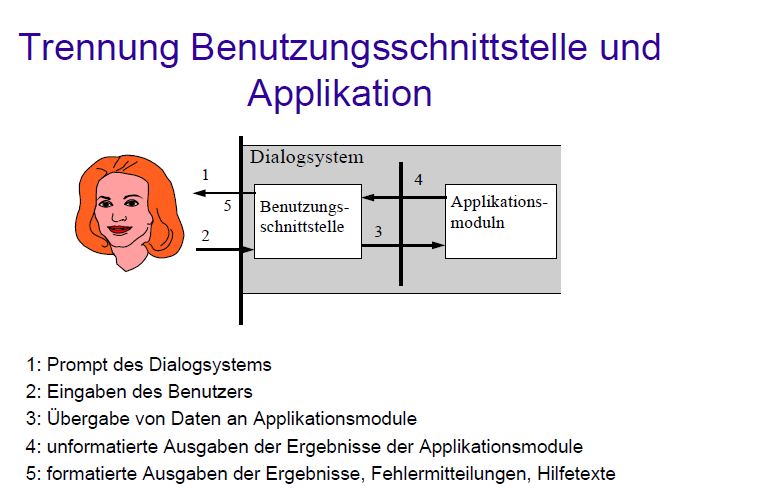
\includegraphics[scale=0.5]{img/ui.png}
	\end{figure}
	
	\item Welche Modelle muss ein Dialogautor beim Entwurf von Benutzungsschnittstellen beachten?
	\begin{itemize}
		\item Benutzermodell -> mentales Modell \\
		Aspekte des Modells: Anwendungsbereich, Arbeitsaufgabe/kontext, kenntnisse, Erfahrungen, Fertigkeiten
		\item Aufgabenmodell -> hauptsächlich HCI im Fokus
		\item Architekturmodell -> UI-Software
		\item Dialogspezifikationsmodell -> siehe Frage vorher(?)
	\end{itemize}
	
	\item Welche Beiträge kann die Ergonomie zur Erstellung von Benutzungsschnittstellen leisten?
	\begin{itemize}
		\item Optimieren der Arbeitsabläufe durch niedrigen Aufwand des Benutzers und hohe Funktionalität des Dialogsystems
		\item ganzheitliche Gestaltung der Software
		\begin{itemize}
			\item benutzergerecht: Berücksichtigung der Stärken und Schwächen des Menschen
			\item aufgabenangemessen: Computer werden vom Benutzer zur Bearbeitung konkreter Aufgaben eingesetzt
			\item technikbewusst: neue technische Optionen zum Wohle des Benutzers einsetzen
			\item organisationsgerecht: Berücksichtigung der organisatorischen Einbindung
		\end{itemize}
		\item Computerwissenschaften -> Softwaredesign -> Dialogtechniken (Informationsdarstellung, Ablauf,..), Software Engineering (Analyse, Modellierung, Entwurf,..), 
		\item Arbeitswissenschaften -> Arbeitsplatzgestaltung; Arbeitspsychologie
		\item Humanwissenschaften -> Physiologie
		\item Psychologie -> Kognition (Gedächtnis, Verstehen, Lernen); Wahrnehmung 
		\item Ergebnisse der Ergonomie:
		\begin{enumerate}
			\item Gesetze und Verordnungen zum Arbeitsschutz
			\item Normen ((inter-)nationale Standards)
			\item Empfehlungen
			\item Designregeln (Gestaltungsregeln, Style Guides, Pattern)
			\item Tools 
		\end{enumerate}
	\end{itemize}
\end{enumerate}


\subsection{Modelle der Human-Computer-Interaction}
Es gibt nicht ein Gesamtmodell, sondern viele Teilmodelle, die in
unterschiedlichen Aspekten hilfreich sein können.
\begin{enumerate}
	\item Was ist ein Dialogsystem?
	siehe subsection vorher
	
	\item Was ist die Benutzungsschnittstelle/User Interface?
	siehe subsection vorher
	
	\item Welche Schnittstellen hat ein Dialogsysteme?
	siehe subsec vorher
	
	\item Welche Modelle müssen Dialogautoren beachten, Welche Rollen gibt es?
	\begin{itemize}
		\item Modelle siehe subsection vorher
		\item Gestalter und Bewerter der physischen Umgebung
		\item Entwickler von UI Tools
		\item Enwickler von UI /Dialogautor
		\item Designer
		\item Bewerter von UI
		\item Applikationsanalysator
		\item Applikationsprogrammierer
		\item ...
		\item Endbenutzer
	\end{itemize}
	
	
	\item Was ist das Seeheim-Modell?
	\begin{itemize}
		\item (ähnlich MVC)
		\item 3 Bestandteile: \\
		Presentation (lexikalische Ebene): für systemnahe Ein/Ausgaben zuständig; verfügt dazu über Devices=Schnittstellen zu physikalischen oder logischen (zb Menüs) Ein/Ausgabegeräten\\
		Dialog control (syntaktische Ebene): durch Austausch von Token Ablauf des Dialogs regeln; unabhängig von Geräte und Anwendung\\
		Applicaiton interface (semantische Ebene): Vermittlerrolle zw. Dialogcontrol und Applikation
		\item Grenzen: Wie erfolgt der Kontrollfluss (siehe nächste Frage)? von welcher Art ist die Kommunikation? (Nachrichtenaustausch oder Prozeduraufruf?)\\
		''schnelle'' grafische Ausgaben brauchen ''Sonderwege'' (wtf?)
	\end{itemize}	
	\begin{figure}[!h]
		\centering
		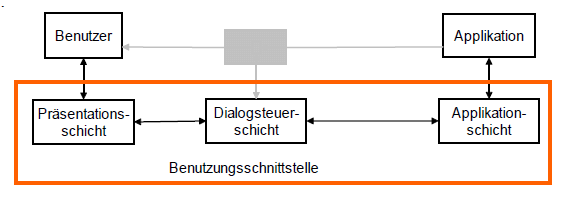
\includegraphics[scale=0.5]{img/seeheim.png}
		\caption{Seeheim Model}
	\end{figure}
	
	\item Welche Vor- und Nachteile haben interne und externe Kontrollarchitekturen
	im Seeheim-Modell?\\
	\textbf{intern:} Programm besitzt alleinige Kontrolle über UI; UI steht als Paket von Unterprogrammen zur Verfügung\\
	\textbf{extern:} Anwendung in Unterprogramme unterteilt, welche von UI aufgerufen werden\\
	\begin{table}[!h]
		\centering
		\begin{tabular}{|p{10em}|p{15em}|p{15em}|}
			\hline
			\hline
			& \textbf{Vorteile} & \textbf{Nachteile}\\
			\hline			
			\textbf{intern} & \tabitem einfache Realisierung & \tabitem keine saubere Aufgabentrennung\\
			&	\tabitem optimale Anpassung an das Anwendungsprogramm & \tabitem bei Änderung an der UI Eingriffe im gesamten Programm\\
			& \tabitem entspricht Vorgehensweise bei Systementwicklungen und Aufgabenzerlegungen & \tabitem sehr lokale Dialoge \\
			&& \tabitem Einheitlichkeit und Konsistenz der UI hängen von Programmierdisziplin ab \\
			\hline
			\hline
			\textbf{extern} &  \tabitem saubere Separierbarkeit von UI und Anwendungsfunktionalität & \tabitem Anwendungsprogramme müssen atomierbar sein\\
			& \tabitem benutzerspezifische UI lässt sich angemessen realisieren & \tabitem Dynamik/Interaktionsfolge liegt außerhalb der Anwendung\\
			& \tabitem anwendungsunabhängige Modifizierbarkeit & Verteilung der Semantik\\
			& \tabitem Leichte Portierbarkeit vom Prototyp zur fertigen Anwendung & \tabitem Komplexität der Schnittstellenbeschreibung\\
			&& \tabitem mögliche Redundanzen in den verschiedenen Unterprogrammen\\
			&& \tabitem Ausgabeaufforderung der Anwendung\\
			\hline
		\end{tabular}
		\caption{Vor- und Nachteile der Kontrollarchitekturen im Seeheim-Modell}
	\end{table}
	
	\item Nennen sie Modelle für Dialogspezifikationen!\\
	dienen zur formalen Spezifikation des Dialogablaufs\\
	sollen ausdrucksstark und einfach sein; typische Dialogstrukturen unterstützen (parallele Prozesse, sequentielle Schritte, Verzweigungen des Ablaufs); unterschiedliche Detailstufen
	\begin{itemize}
		\item Multi-Party-Grammatiken: kontextfreie Grammatiken; Erweiterung der BNF durch Spezifikation wer was tut bei Interaktion; einfach und natürlich, aber nicht ausdrucksstark
		\item Menühierarchien: baumartige Struktur zur Spezi von Alternativen; einfach, aber nicht ausdrucksstark
		\item Zustandsübergangsdiagramme (STN): quasi Graph der Transitionen darstellt
		\item verbesserte STN (=ATN)
		\item State Charts: lösen einige Probleme der STN/ATN, zb Hierarchische, nebenläufige, Zustände, History
		\item Ereignis Handler: Dialogbeschreibung durch Regeln
		\item Petri-Netze: sollte klar sein
		\item User-Action-Notation
	\end{itemize}
		
	\item Welche Benutzermodelle kennen sie?\\
	Ziel: konsistentes Dialogverhalten auch in breitem Anwendungsbereich anhand Wissen des Nutzers über Anwendungsbereich, seine Ziele und seine Pläne\\
	Einteilung nach Datenverarbeitungskenntnissen (DV):
	\begin{itemize}
		\item Anfänger
		\item gelegentlicher Nutzer
		\item Experte
	\end{itemize}
		
	\item Welche Benutzerklassen sollten unterschieden werden?\\
	Kriterien zur Unterscheidung von Benutzern
	\begin{itemize}
		\item \textbf{Vorwissen/Fachliche Erfahrung:} zum Anwendungsgebiet -> mit Erfahrung geht Anwender mit Erwartungen an neues Tool
		\item \textbf{Vertrautheit:} mit Begriffen und Konzepten der DV prägen das Verhalten beim Dialog
		\item \textbf{Kognitive Fähigkeiten:} Stil der Problemlösung, Experimentierfreudigkeit oder Ägnstlichkeit beschleunigen oder verzögern das Lernverhalten
		\item \textbf{Einstellungen:} ggüber Dialogsystemen können Effektivität beeinflussen -> grundsätzliche Haltung ggüber Computern; persönliche Gründe für das Arbeiten (freiwillig - zwang; privat - beruflich)
		\item \textbf{Persönliche Ziele:} beim Erlernen der Bedienung des Systems -> vorrangig ist Arbeitsaufgabe, Beherrschen der Systeme nur soweit wie nötig ODER primäres Ziel ist Verstehen und Beherrschen des Systems
	\end{itemize}
	
	\item Was sind Personas?\\	
	beschreiben fiktive Benutzer als Stereotyp und Referenzperson zur Analyse und Definition von Anforderungen an interaktive Systeme -> Stereotyp zwingt zum Nachdenken über konkrete statt allgemeine Nutzer
	
	\item Erläutern sie das Model-View-Controller- Modell!
	\begin{itemize}
		\item entstanden als Experiment aus Seeheim Modell
		\item Aufteilung in Klassen - MVC halt..
		\item Vorteile: problemlose Integration in OO Entwurf; problemlose Anpassung an unterschiedliche Benutzer; Unterstützung unterschiedlicher Sichten auf Daten
		\item Probleme: MVC als alleiniges Architekturmodell nicht geeignet; Trennung Ctrl - View oft nicht zweckmäßig
	\end{itemize}
	
	\item Wozu dienen GOMS-Modelle?
	\begin{itemize}
		\item \textbf{G}oals: eine Menge von Zielen
		\item \textbf{O}perators: Menge von Operationen
		\item \textbf{M}ethods: Menge von Methoden zum Erreichen von Zielen
		\item \textbf{S}election rules: Menge von Auswahlregeln von Methoden
		\item geht von geübten Nutzern aus, d.h. jene die das System bereits kennen
		\item Modell erlaubt Abschätzungen oder Vorhersagen des Lernaufwandes für den Erwerb des prozeduralen Benutzerwissens
		\item zusätzliche Vorhersagen für Ausführungsaufwand und Performanz 
		\item Kritik: Berücksichtigt nicht Ermüdung des Nutzers, soziales organisatorisches Umfeld, Unberechenbarkeit des Nutzers, Gewohnheiten/Vorlieben des Nutzers
	\end{itemize}
\end{enumerate}